\section{Results}

\subsection{Computational platform and Software Environment}

This evaluation was performed on the NERSC Perlmutter supercomputer using two AMD EPYC 7763 processors with a base clock speed of 2.45~GHz. The system was configured with 512~GB of DDR4 memory per node, a 32~KB L1 cache, a 512~KB L2 cache, and a 32~MB L3 cache, providing ample resources for large matrix multiplications. The operating system is SUSE Linux Enterprise Server 15~SP6 with kernel version \texttt{6.4.0\char45 150600.23.125\_15.0.29\char45 cray}\\ \texttt{\detokenize{_shasta_c}}. GCC 14.3.0 and CMake 3.28.3 were used for compilation and build configuration, respectively. \cite{nersc}

\subsection{Methodology}

While conducting this evaluation, we focused on measuring the performance of our matrix multiplication implementations under various configurations. We utilized OpenMP for parallelization and compared the performance of our Basic Matrix Multiplication, Blocked Matrix Multiplication, and the CBLAS library. The evaluation was conducted across different problem sizes, specifically 128, 512, and 2048, to assess scalability and efficiency. We collected data on execution time, speedup, and cache access patterns to provide a comprehensive understanding of the performance characteristics of each implementation.

All metrics were collected using the job files which leveraged the LIKWID performance monitoring tool, allowing us to capture detailed information about speedup using the Runtime (RDTSC) values as well as cache access patterns using the L2 and L3 cache access counters. The collected data was then analyzed to identify trends, bottlenecks, and areas for optimization.

\subsection{Scaling Study for Basic MM with OpenMP parallelization}

The scaling study for basic matrix multiplication with OpenMP parallelization was conducted to evaluate the performance improvements achieved through parallel execution. The study involved running the Basic MM implementation across different problem sizes and measuring the speedup achieved by utilizing multiple threads.

To collect this data, we executed the included job-basic-omp file, which was designed to run the Basic MM implementation with OpenMP parallelization. The job file was configured to utilize multiple threads, allowing us to observe the performance gains achieved through parallel execution.

The problem sizes tested were 128, 512, and 2048, and the speedup was calculated by comparing the execution time of the parallel implementation against the serial version. The results of this scaling study are presented in Figure~\ref{fig:basic_openmp_comparison}, which illustrates the speedup achieved for each problem size.

Speedup was calculated using the formula:
\begin{equation}
    \text{Speedup} = \frac{\text{Execution Time (Serial)}}{\text{Execution Time (Parallel)}}
\end{equation}

The execution time for the parallel implementation was measured using the maximum runtime recorded across all threads, while the serial execution time was obtained from the single-threaded execution of the Basic MM implementation. The reason for using the maximum runtime across threads is to account for the fact that the overall execution time is determined by the slowest thread, which can be influenced by factors such as load imbalance and thread synchronization overhead.

Figure~\ref{fig:basic_openmp_comparison} shows the speedup by problem size for the basic matrix multiplication implementation parallelized with OpenMP.

\begin{figure}[H]
    \centering
    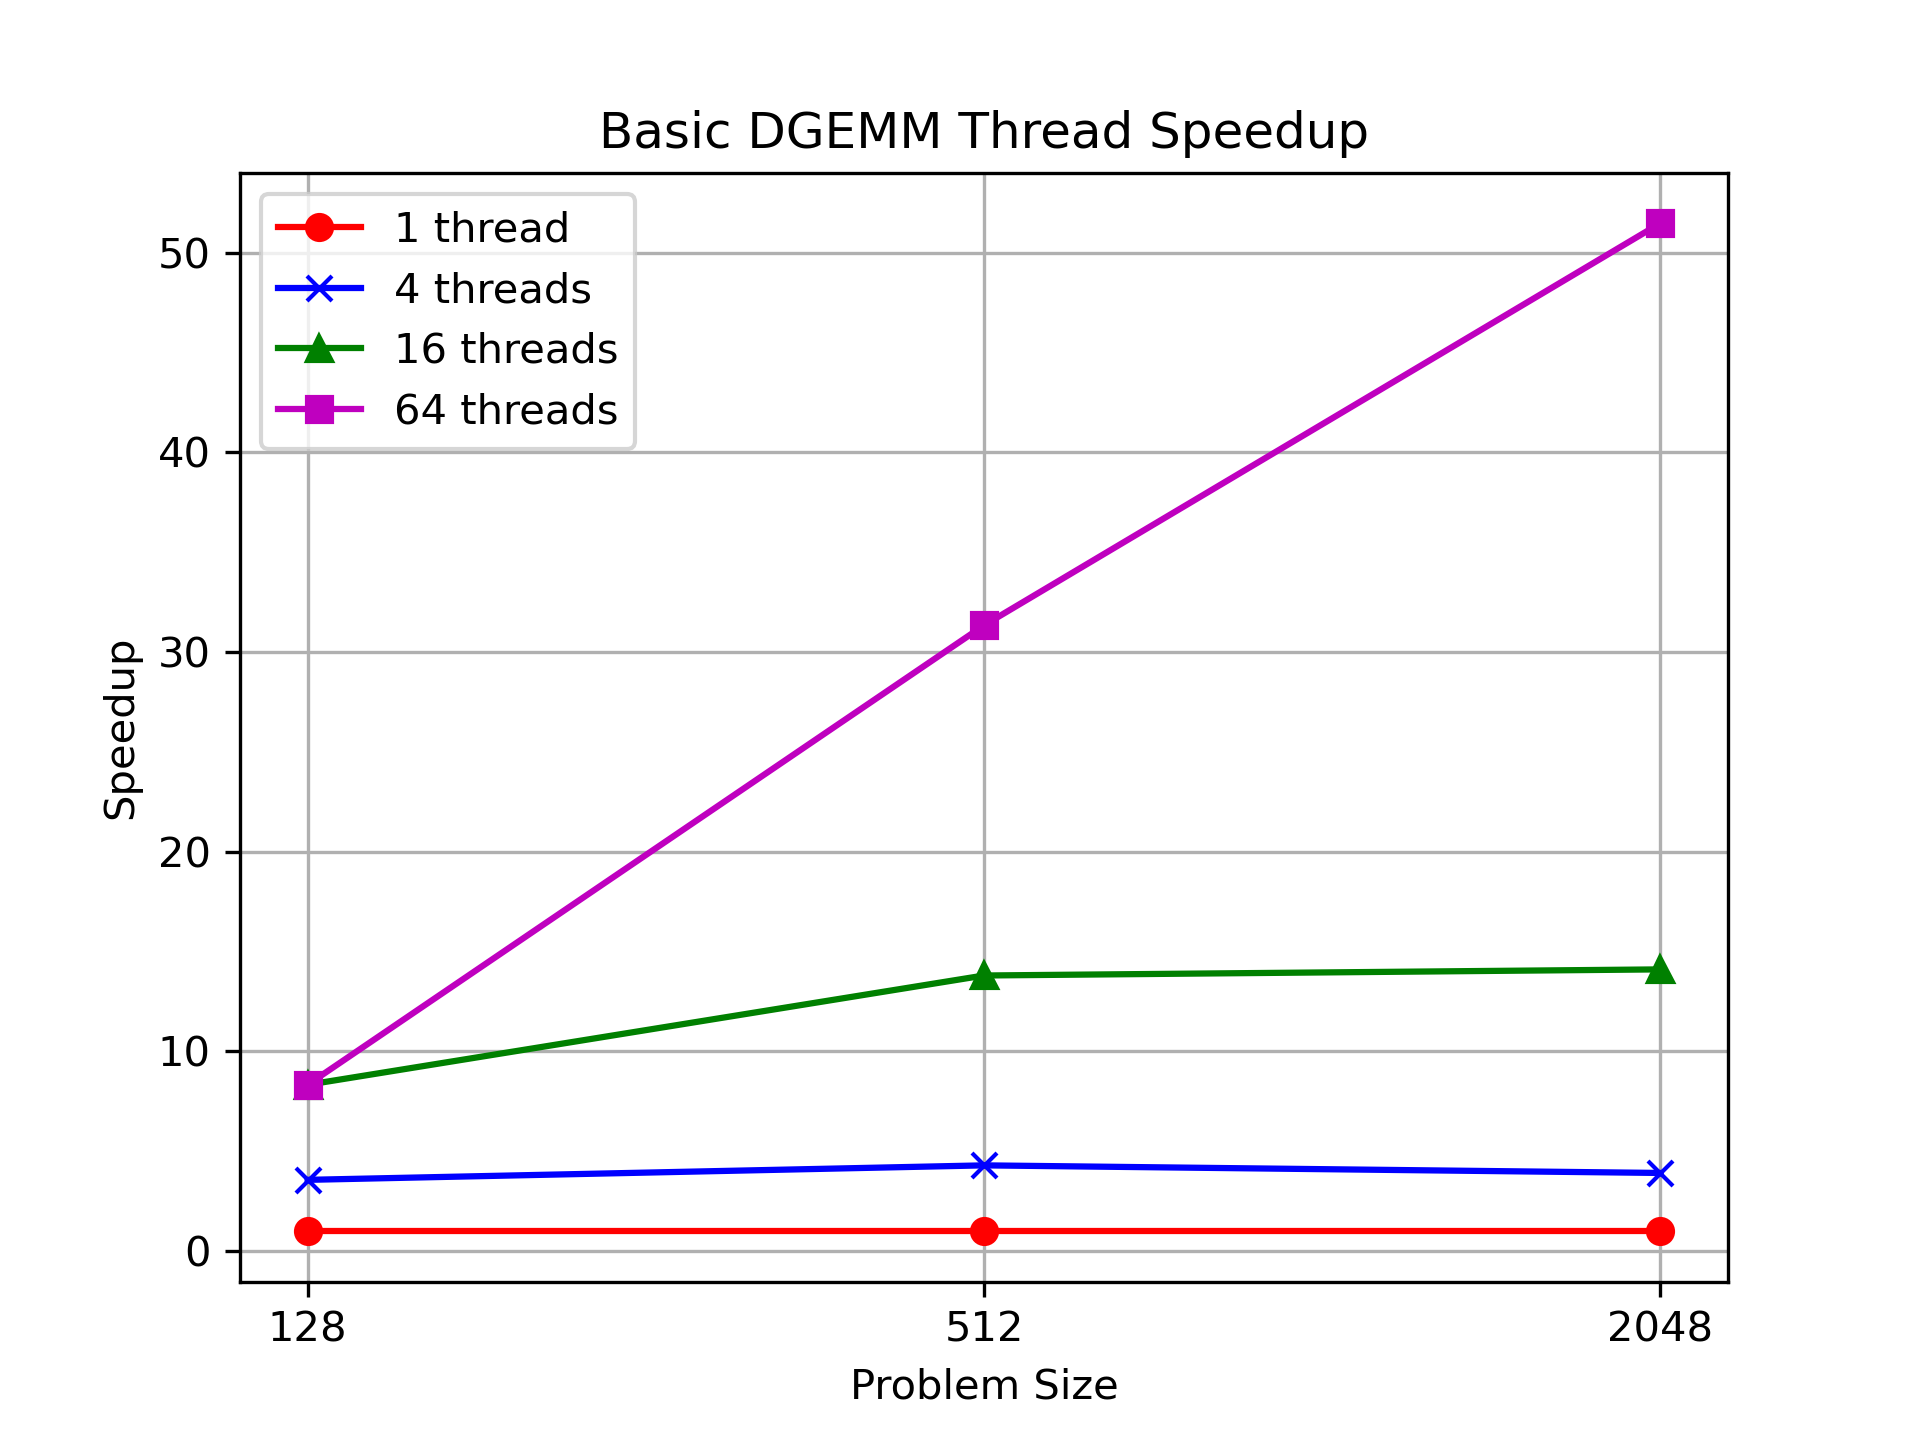
\includegraphics[width=.75\linewidth]{images/basic_speedup.png}
    \caption{Speedup of Basic Matrix Multiplication with OpenMP parallelization}
    \label{fig:basic_openmp_comparison}
\end{figure}

We observed that the speedup achieved by the Basic implementation was significant as concurrency increased, with the highest speedup observed for the largest problem size of 2048 and a concurrency of 64 threads. We also observed that speedup was not linear as well and see that problem size seems to have the most significant increases on the 64-thread speedup. This is likely due to the greater ability to utilize the available threads for larger problem sizes.

\subsection{Evaluation of BMMCO with OpenMP parallelization}

For the blocked matrix multiplication implementation with OpenMP parallelization, we conducted a similar scaling study to evaluate its performance improvements. The study involved running the blocked implementation across different problem sizes and measuring the speedup achieved by utilizing multiple threads.

To collect this data, we executed the included job-blocked-omp file, which was designed to run the blocked implementation with OpenMP parallelization. The job file was configured to utilize multiple threads, allowing us to observe the performance gains achieved through parallel execution.

To calculate speedup, we used the same formula as in the previous section, comparing the execution time of the parallel implementation against the serial version. The execution time for the parallel implementation was measured using the maximum runtime recorded across all threads, while the serial execution time was obtained from the single-threaded execution of the blocked implementation.

Figure~\ref{fig:blocked_openmp_comparison} shows the speedup by problem size for the blocked implementation parallelized with OpenMP. 

 \begin{figure}[H]
    \centering
    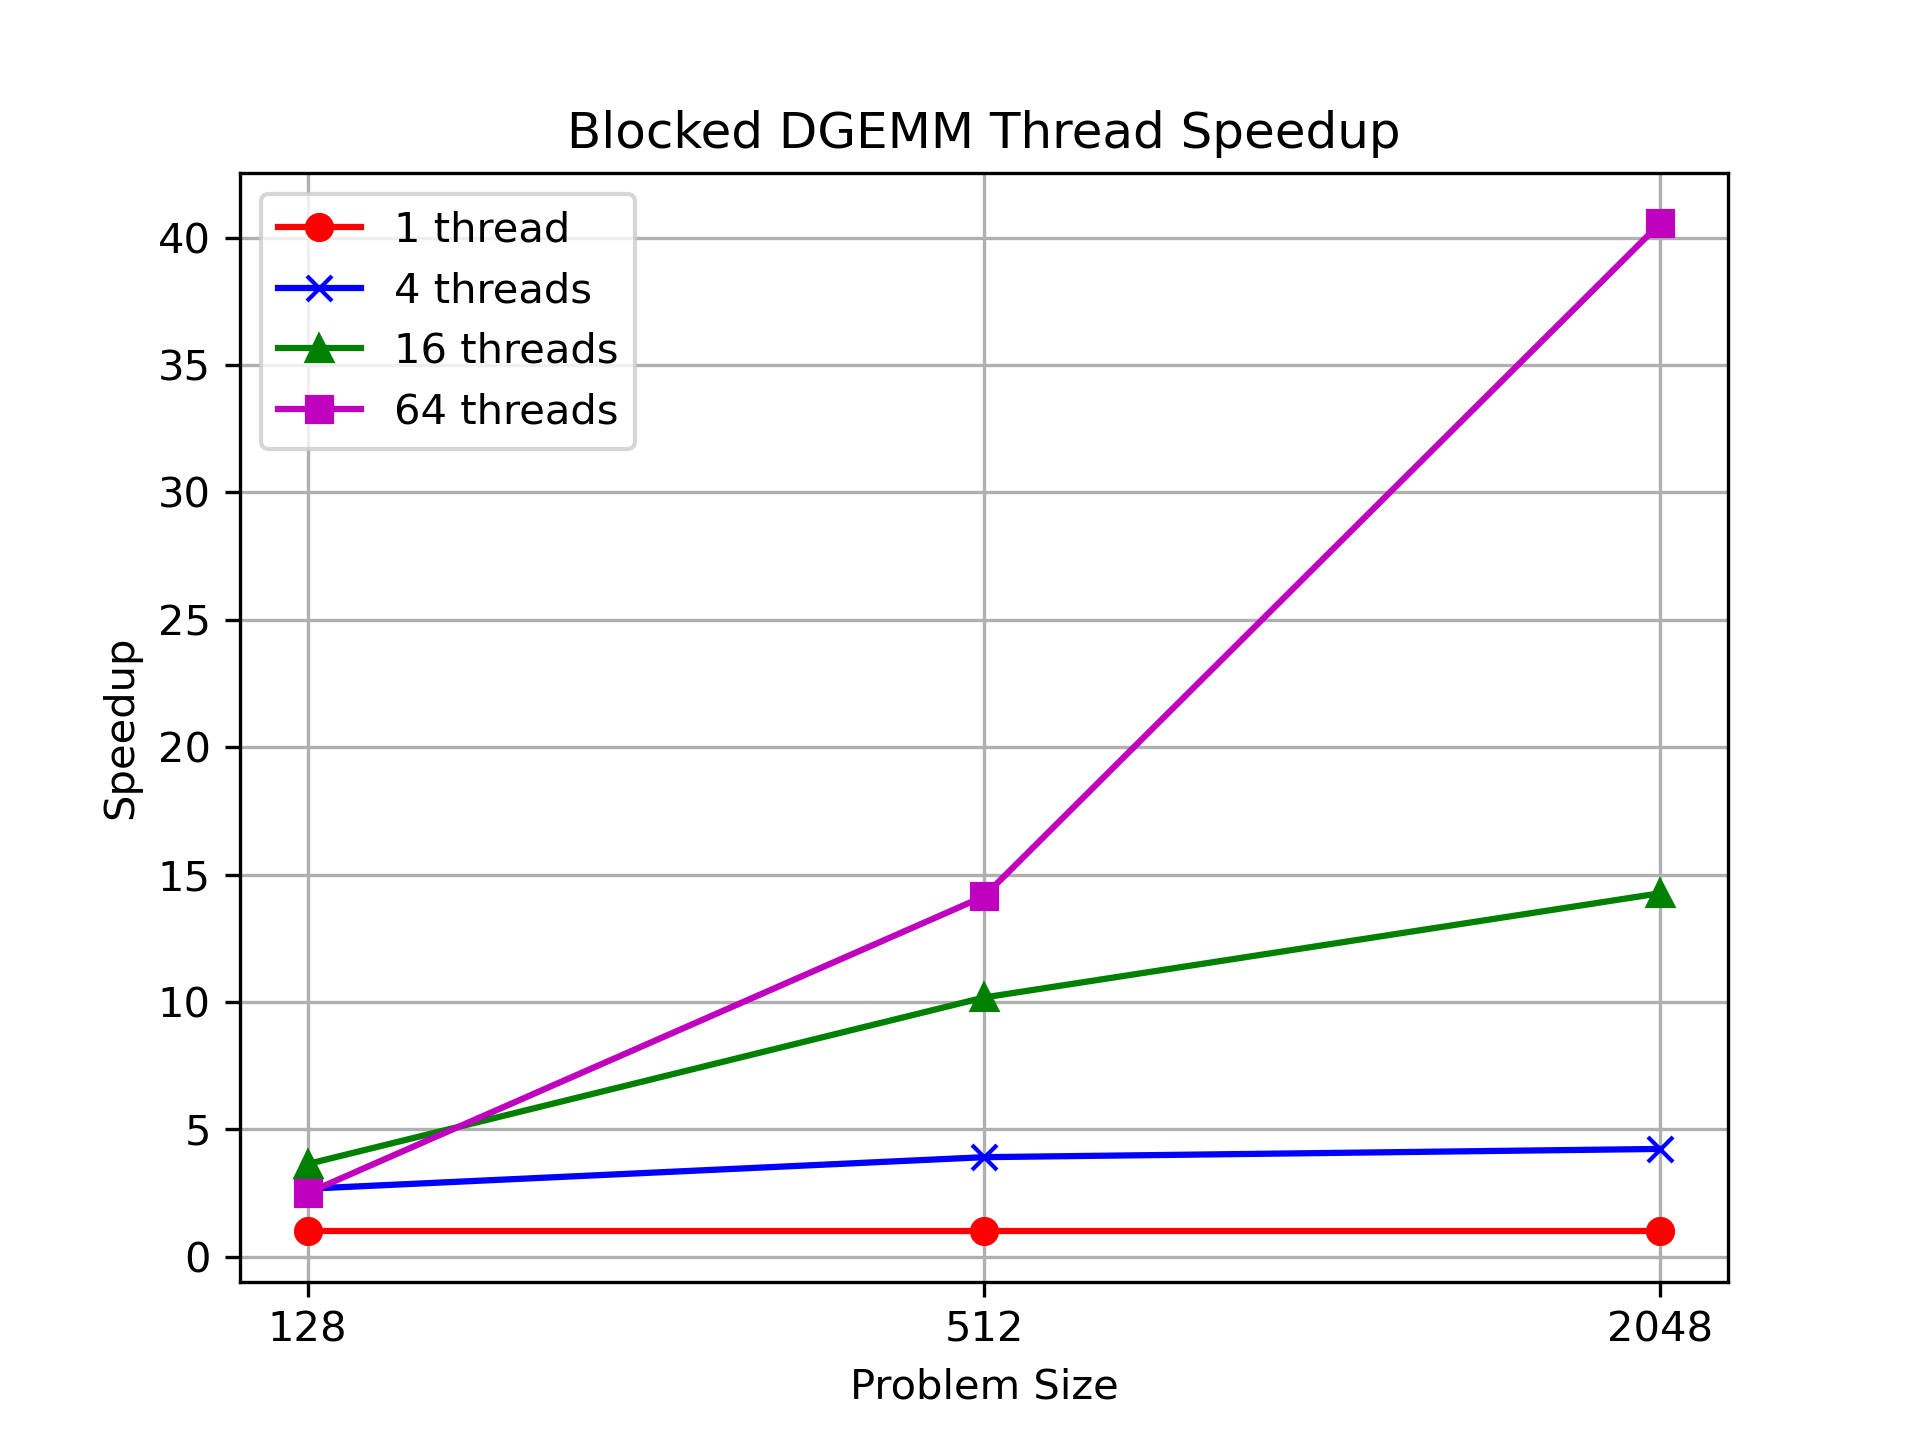
\includegraphics[width=.75\linewidth]{images/blocked_speedup.png}
    \caption{Speedup of Blocked Matrix Multiplication with OpenMP parallelization}
    \label{fig:blocked_openmp_comparison}
\end{figure}

In this observation, we found that speedup was less significant for the blocked implementation compared to the basic implementation. The highest speedup was observed for the largest problem size of 2048 and a concurrency of 64 threads, but the overall speedup was lower than that of the basic implementation. Additionally, we observed that the different problem sizes had generated elevated speedup for the threads less than 64 when compared tot the basic implementation.

The lower overall speedup for the blocked implementation can be attributed to the increased complexity of the algorithm compared to the basic implementation, which may introduce additional computational overhead.

\subsection{Comparison of CBLAS, BasicMM-omp, and BMMCO-omp}

\begin{table}[H]
    \centering
    \caption{Normalized L2 cache accesses. Each value is divided by the
    corresponding CBLAS L2 access count for the same problem size.}
    \label{tab:normalized_l2_accesses}
    \small
    \begin{tabular}{@{}rcccc@{}}
        \toprule
        Problem size & CBLAS & Basic & Blocked B4 & Blocked B16 \\
        \midrule
        128  & 1.000 & 44.987  & 4.574  & 1.335 \\
        512  & 1.000 & 45.813  & 4.449  & 1.977 \\
        2048 & 1.000 & 120.906 & 7.807  & 2.013 \\
        \bottomrule
    \end{tabular}
\end{table}

\begin{table}[H]
    \centering
    \caption{Normalized L3 cache accesses. Each value is divided by the
    corresponding CBLAS \texttt{L3\_ACCESS\_ALL\_TYPES} count for the same
    problem size.}
    \label{tab:normalized_l3_accesses}
    \small
    \begin{tabular}{@{}rcccc@{}}
        \toprule
        Problem size & CBLAS & Basic & Blocked B4 & Blocked B16 \\
        \midrule
        128  & 1.000 & 0.044   & 0.035  & 0.053 \\
        512  & 1.000 & 273.351 & 13.936 & 3.043 \\
        2048 & 1.000 & 604.116 & 20.994 & 4.508 \\
        \bottomrule
    \end{tabular}
\end{table}


\subsection{Overall findings and discussion}

